
\section{Engenharia de Software}

\begin{frame}
\frametitle{Objetivos}
\begin{itemize}
 \item Identificar as atividades para auxiliar a compreensão e resolução de probblemas da engenharia de software
 %\pause
 \item Explicar as boas práticas
 %\pause
 \item Apresentar o RUP no contexto das boas práticas.
\end{itemize}
\end{frame}

\begin{frame}
 \frametitle{Conteúdo}
 \begin{itemize}
  \item Os problemas do desenvolvimento de software
  \begin{itemize}
   \item As seis boas práticas
  %\pause
   \item O RUP no contexto das boas práticas
  \end{itemize}
 \end{itemize}
\end{frame}

\begin{frame}
 \frametitle{Sintomas dos problemas do desenvolvimento de Software}
 \begin{itemize}
  \item Necessidades desconhecidas
  %\pause
  \item Requisitos mal especificados
  %\pause
  \item Módulos não se integram
  %\pause
  \item Dificuldade de manutenção
  %\pause
  \item Descoberta tardia dos defeitos
  %\pause
  \item Pouca experiência do usuário final
  %\pause
  \item Baixo desempenho
  %\pause
  \item Esforços não coordenados da equipe
  %\pause
  \item Problemas na homologação
 \end{itemize}	
\end{frame}

\begin{frame}
 \frametitle{Rastreie os Sintomas das Causas Raízes}
  \begin{figure}
   \centering
   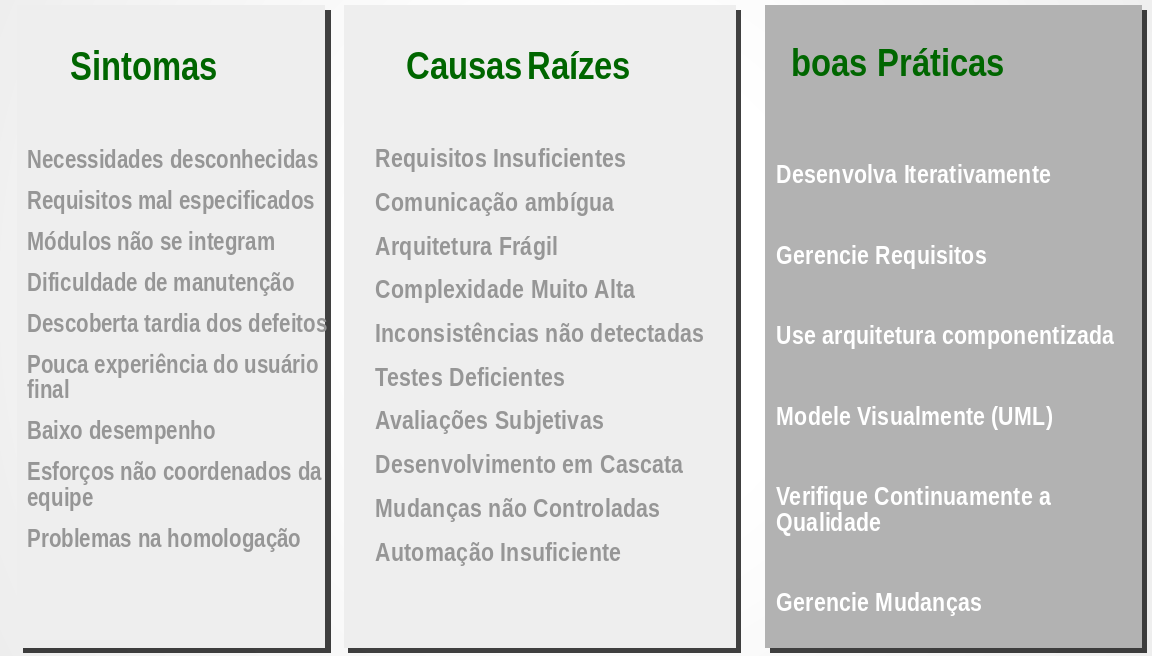
\includegraphics[width = 0.9\textwidth]{figs/fig5.png}
  \end{figure}
\end{frame}

\begin{frame}
 \frametitle{Rastreie os Sintomas das Causas Raízes}
  \begin{figure}
   \centering
   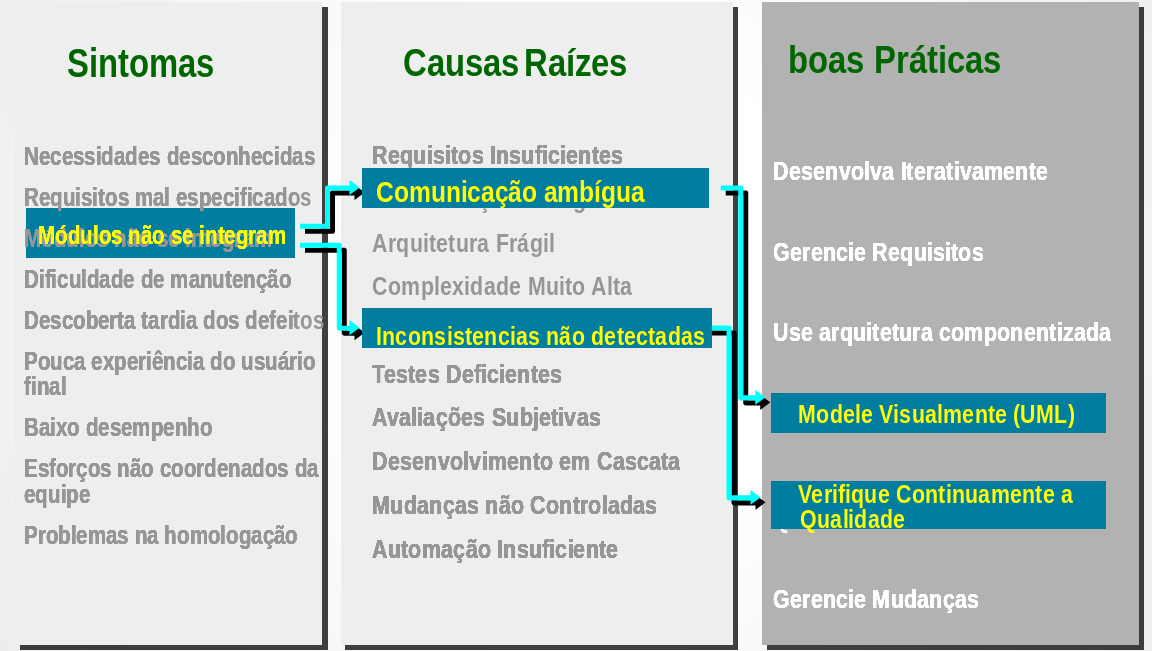
\includegraphics[width = 0.9\textwidth]{figs/fig6.png}
  \end{figure}
\end{frame}
\section{Desenvolva Iterativamente}
\begin{frame}
 \frametitle{Prática 1: Desenvolva Iterativamente}
 \begin{block}{Boas Práticas}
 \begin{itemize}
  \item \textbf{Desenvolva Iterativamente}
  \item Gerencie Requisitos
  \item Use arquitetura componentizada
  \item  Modele Visualmente (UML)
  \item  Verifique Continuamente a Qualidade
  \item Gerencie Mudanças  
 \end{itemize}
\end{block}
\end{frame}

\begin{frame}
 \frametitle{Características do Desenvolvimento em Cascata}
 \begin{minipage}[t]{0.48\linewidth}
  \begin{itemize}
   \item Confirmação tardia da resolução dos riscos
    %\pause
    \item Progresso medido por meio de produtos que possuem baixa qualidade
    %\pause
    \item Atrasos e "remendos" no produto
    %\pause
    \item Frequentemente resulta em iterações não planejadas
  \end{itemize}
 \end{minipage}
\begin{minipage}[t]{0.48\linewidth}
\textbf{Processo em Cascata}
  \begin{figure}
   \centering
   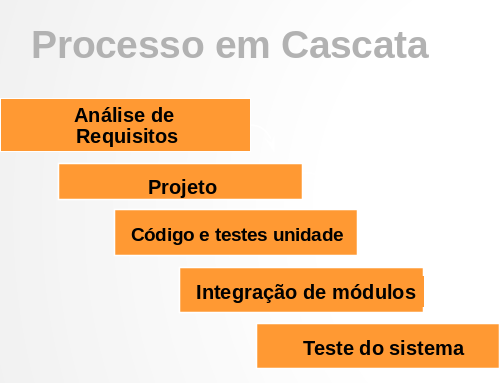
\includegraphics[width = 0.8\textwidth]{figs/fig7.png}
  \end{figure}
\end{minipage}
\end{frame}


\begin{frame}
 \frametitle{Desenvolvimento iterativo produz releases}
  \begin{figure}
   \centering
   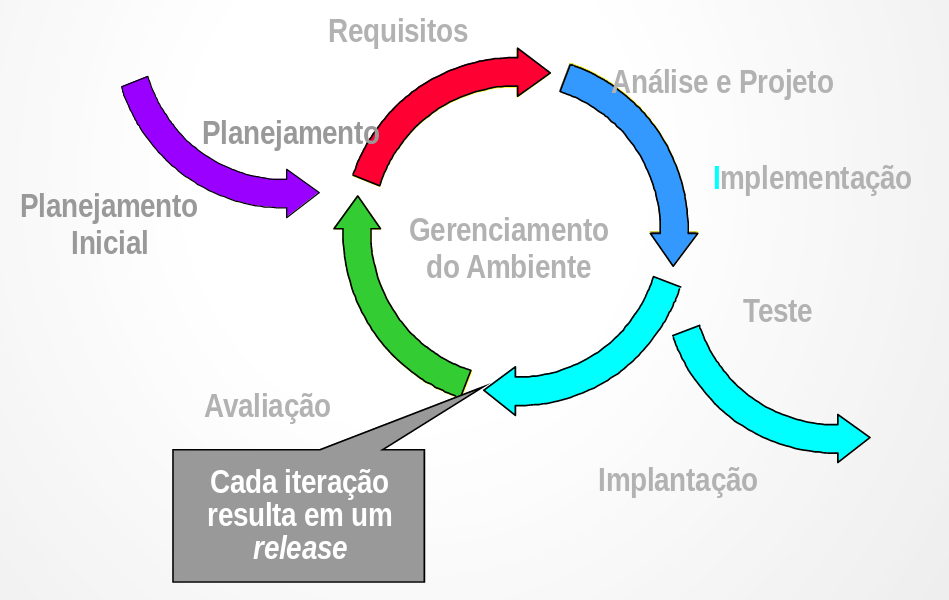
\includegraphics[width = 0.9\textwidth]{figs/fig8.png}
  \end{figure}
\end{frame}

\begin{frame}
 \frametitle{Desenvolvimento iterativo produz releases}
\begin{block}{Wikipedia}
 Uma liberação ou lançamento de software (em inglês: "release") refere-se ao lançamento de uma nova versão oficial de um produto de software
\end{block}

\end{frame}


\begin{frame}
 \frametitle{Perfil de Risco}
  \begin{figure}
   \centering
   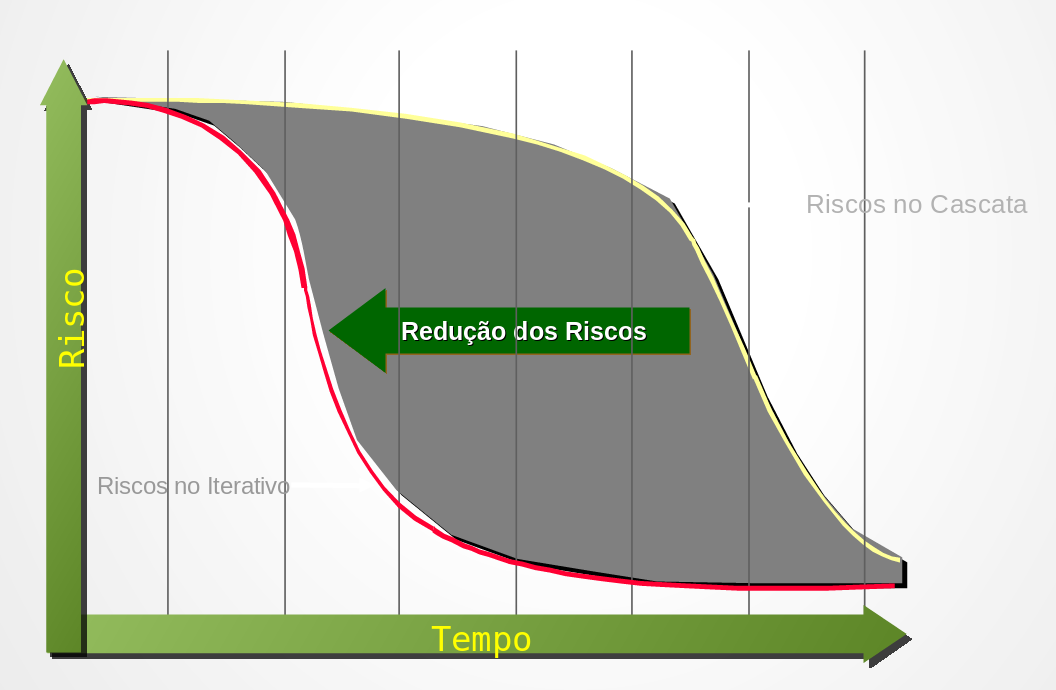
\includegraphics[width = 0.9\textwidth]{figs/fig9.png}
  \end{figure}
\end{frame}
\section{Gerencie Requisitos}
\begin{frame}
 \frametitle{Prática 2: Gerencie Requisitos}
 \begin{block}{Boas Práticas}
 \begin{itemize}
  \item Desenvolva Iterativamente
  \item \textbf{Gerencie Requisitos}
  \item Use arquitetura componentizada
  \item  Modele Visualmente (UML)
  \item  Verifique Continuamente a Qualidade
  \item Gerencie Mudanças  
 \end{itemize}
\end{block}
\end{frame}

\begin{frame}
 \frametitle{Gerenciamento de Requisitos}
 \begin{itemize}
  \item Tenha certeza que
  \begin{itemize}
   \item está resolvendo o problema correto
   \item está construindo os “builds” corretos
  \end{itemize}
  \item por meio de uma abordagem sistemática
  \begin{itemize}
   \item de levantamento dos problemas
   \item organizada
   \item documentada
   \item gerenciada 
   \end{itemize}

 \end{itemize}

\end{frame}

\begin{frame}
 \frametitle{Aspectos da gerência de requisitos}
 \begin{itemize}
  \item Analise o problema
  \item Entenda as necessidades do usuário
  \item Defina o sistema
  \item Gerencie o escopo
  \item Refine a definição do problema
  \item Gerencie a mudança dos requisitos
 \end{itemize}
\end{frame}

\begin{frame}
 \frametitle{Mapa do território dos requisitos}
  \begin{figure}
   \centering
   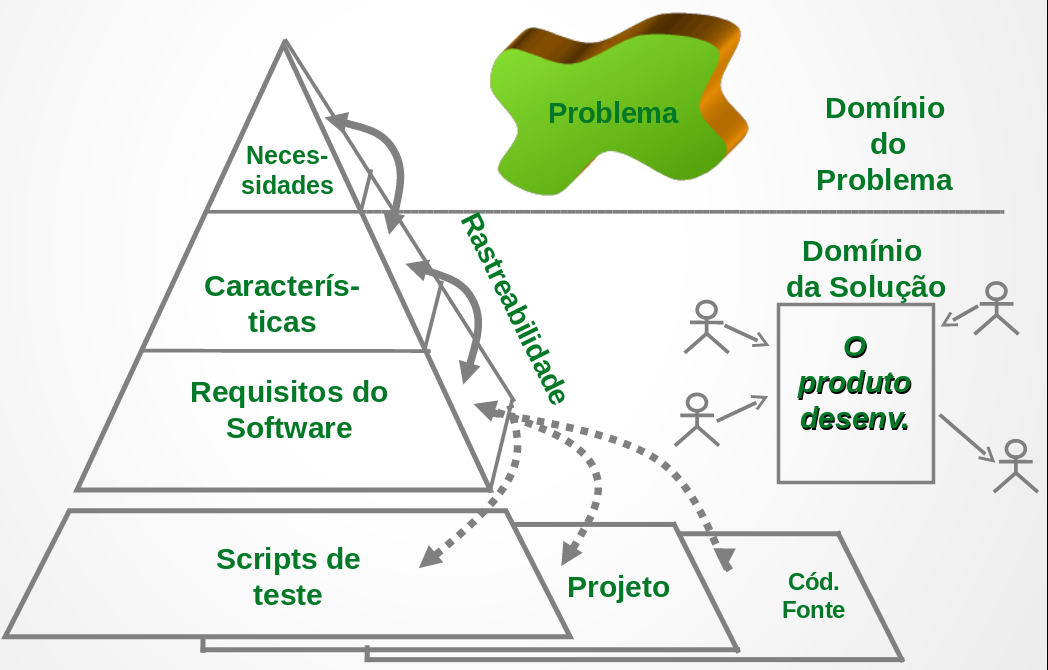
\includegraphics[width = 0.9\textwidth]{figs/fig10.png}
  \end{figure}
\end{frame}



\section{Arquitetura componentizada}
\begin{frame}
 \frametitle{Prática 3: arquitetura componentizada}
 \begin{block}{Boas Práticas}
 \begin{itemize}
  \item Desenvolva Iterativamente
  \item Gerencie Requisitos
  \item \textbf{Use arquitetura componentizada}
  \item  Modele Visualmente (UML)
  \item  Verifique Continuamente a Qualidade
  \item Gerencie Mudanças  
 \end{itemize}
\end{block}
\end{frame}

\begin{frame}
 \frametitle{Componente de Software}
 \begin{block}{Definição}
  é o termo utilizado para descrever o elemento de software que encapsula uma série de funcionalidades. 
  Um componente é uma unidade independente, que pode ser utilizado com outros componentes para formar um sistema mais complexo.
 \end{block}
\footnote{Fonte: Wikipedia}
\end{frame}

\begin{frame}
 \frametitle{Arquitetura robusta baseada em componentes}
 \begin{itemize}
  \item Robustez
  \begin{itemize}
   \item Conhece os requisitos atuais e futuros
    \item Melhora a extensibilidade
    \item Promove o reuso
    \item Encapsula as dependências do sistema
  \end{itemize}
  \item Baseada em Componentes
  \begin{itemize}
   \item Reusa ou customiza os componentes
    \item Seleciona componentes comercialmente disponíveis
    \item Envolva o legado de forma incremental
  \end{itemize}
 \end{itemize}
\end{frame}

\begin{frame}
 \frametitle{Propóstio de uma arquitetura robusta baseada em componentes}
  \begin{minipage}[t]{0.48\linewidth}
  \begin{itemize}
   \item Base para o reuso
   \begin{itemize}
    \item Reuso de componentes
    \item Reuso da arquitetura
   \end{itemize}
  \item Base para o gerenciamento de projetos
  \begin{itemize}
   \item Planejamento
   \item Staffing
   \item Entregas
  \end{itemize}
  \item Controle intelectual
  

  \end{itemize}
 \end{minipage}
\begin{minipage}[t]{0.48\linewidth}
\begin{itemize}
   \item Gerencia da complexidade
    \item Mantém a integridade
  \end{itemize}
  \begin{figure}
   \centering
   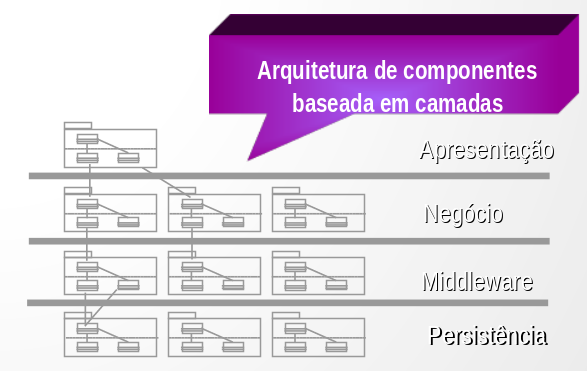
\includegraphics[width = 0.9\textwidth]{figs/fig11.png}
  \end{figure}
\end{minipage}

\end{frame}

\section{Modele Visualmente (UML)}
\begin{frame}
 \frametitle{Prática 3: Modele Visualmente (UML)}
 \begin{block}{Boas Práticas}
 \begin{itemize}
  \item Desenvolva Iterativamente
  \item Gerencie Requisitos
  \item Use arquitetura componentizada
  \item  \textbf{Modele Visualmente (UML)}
  \item  Verifique Continuamente a Qualidade
  \item Gerencie Mudanças  
 \end{itemize}
\end{block}
\end{frame}

\begin{frame}
 \frametitle{Por que modelar visualmente?}
 \begin{itemize}
  \item Capturar a estrutura e comportamento
  \item Mostrar como os elementos do sistema se integram
  \item Manter o projeto e implementação
  \item Expor ou esconder apropriadamente os detalhes
  \item Promover comunicação sem ambuiguidade
  \item Prover uma linguagem comum a equipe por meio da UML
 \end{itemize}
\end{frame}

\begin{frame}
 \frametitle{Modelagem Visual com a \textbf{U}nified \textbf{M}odeling \textbf{L}anguage}
 \begin{itemize}
  \item Múltiplas Visões
  \item Sintaxe e semântica precisas
 \end{itemize}
  \begin{figure}
   \centering
   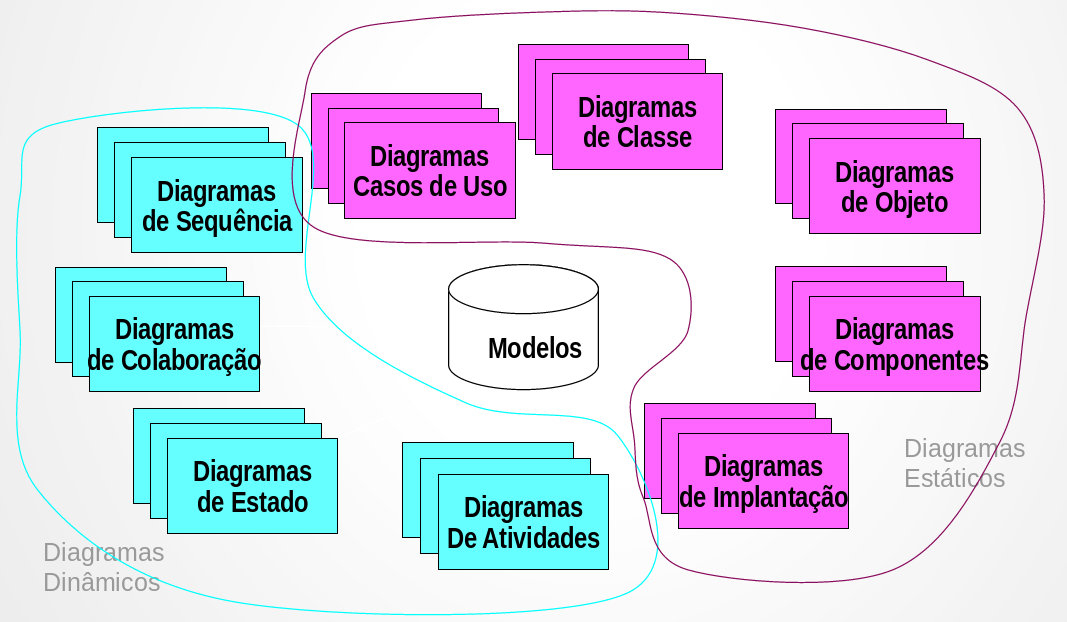
\includegraphics[width = 0.8\textwidth]{figs/fig12.png}
  \end{figure}
\end{frame}

\begin{frame}
 \frametitle{Modelagem Visual com Diagramas UML}
 
  \begin{figure}
   \centering
   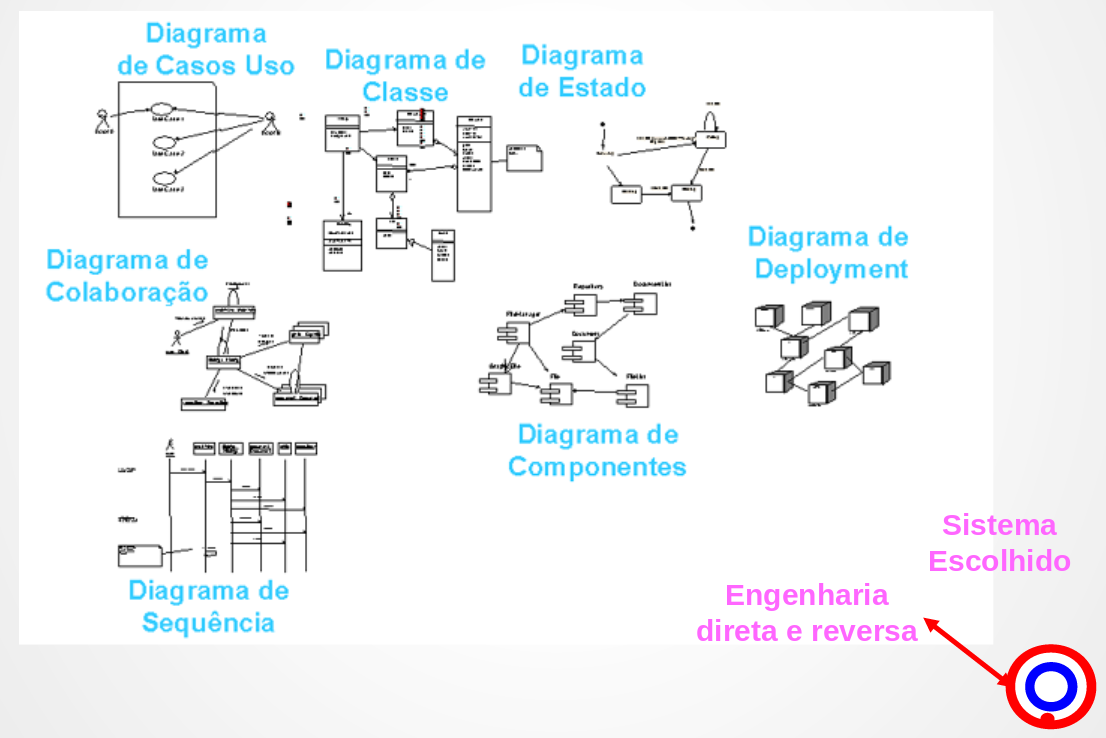
\includegraphics[width = 0.9\textwidth]{figs/fig13.png}
  \end{figure}
\end{frame}

\section{ Verifique Continuamente a Qualidade}
\begin{frame}
 \frametitle{Prática 3:  Verifique Continuamente a Qualidade}
 \begin{block}{Boas Práticas}
 \begin{itemize}
  \item Desenvolva Iterativamente
  \item Gerencie Requisitos
  \item Use arquitetura componentizada
  \item  Modele Visualmente (UML)	
  \item  \textbf{Verifique Continuamente a Qualidade}
  \item Gerencie Mudanças  
 \end{itemize}
\end{block}
\end{frame}

\begin{frame}
\frametitle{Verifique Continuamente a Qualidade do seu Software}
 \begin{itemize}
  \item Problemas em Software são de 100 a 1000 vezes mais caros para serem  encontrados e corrigidos após a implantação
 \end{itemize}
\begin{figure}
   \centering
   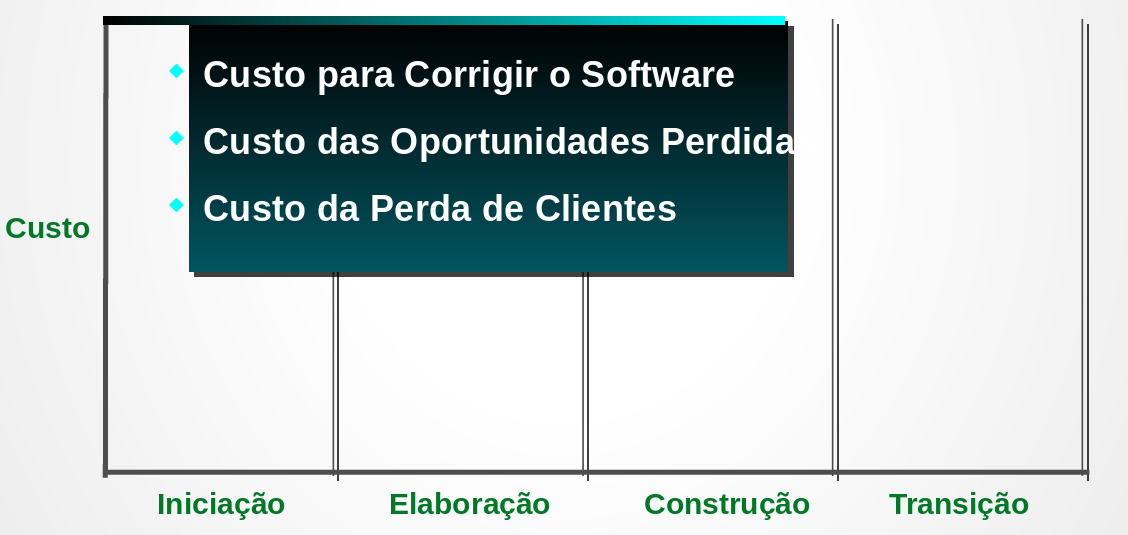
\includegraphics[width = 0.9\textwidth]{figs/fig14.png}
  \end{figure}
\end{frame}


\begin{frame}
\frametitle{Dimensões de Qualidade do Teste}
\begin{figure}
   \centering
   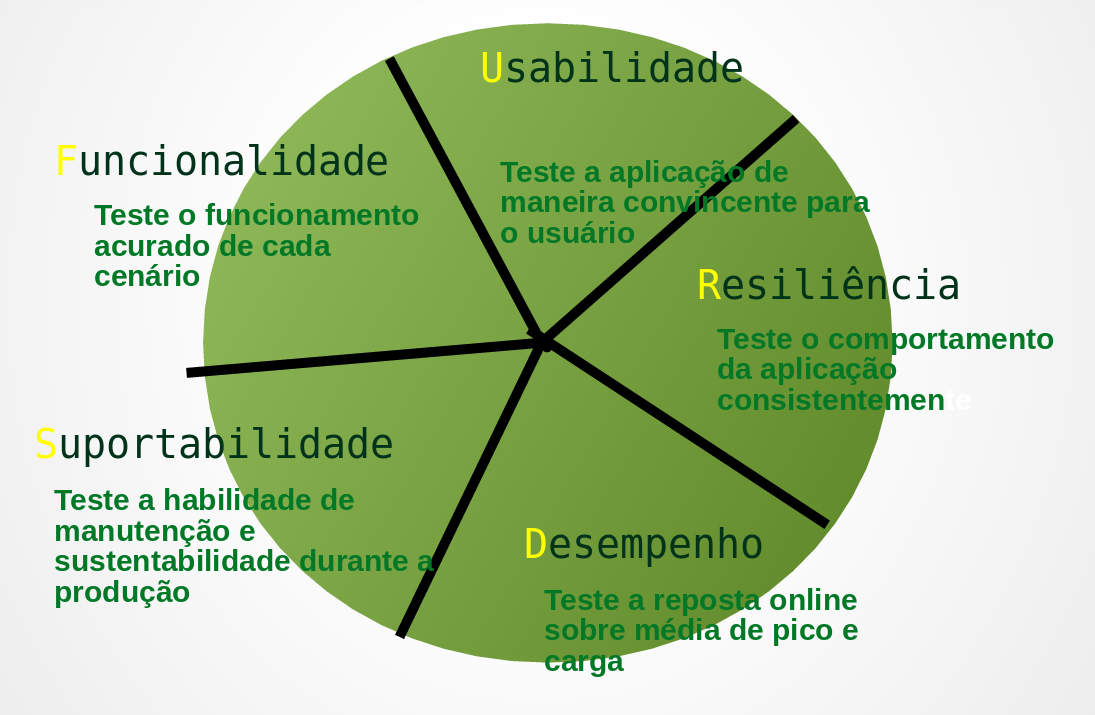
\includegraphics[width = 0.9\textwidth]{figs/fig15.png}
  \end{figure}
\end{frame}


\begin{frame}
\frametitle{Teste cada iteração}
\begin{figure}
   \centering
   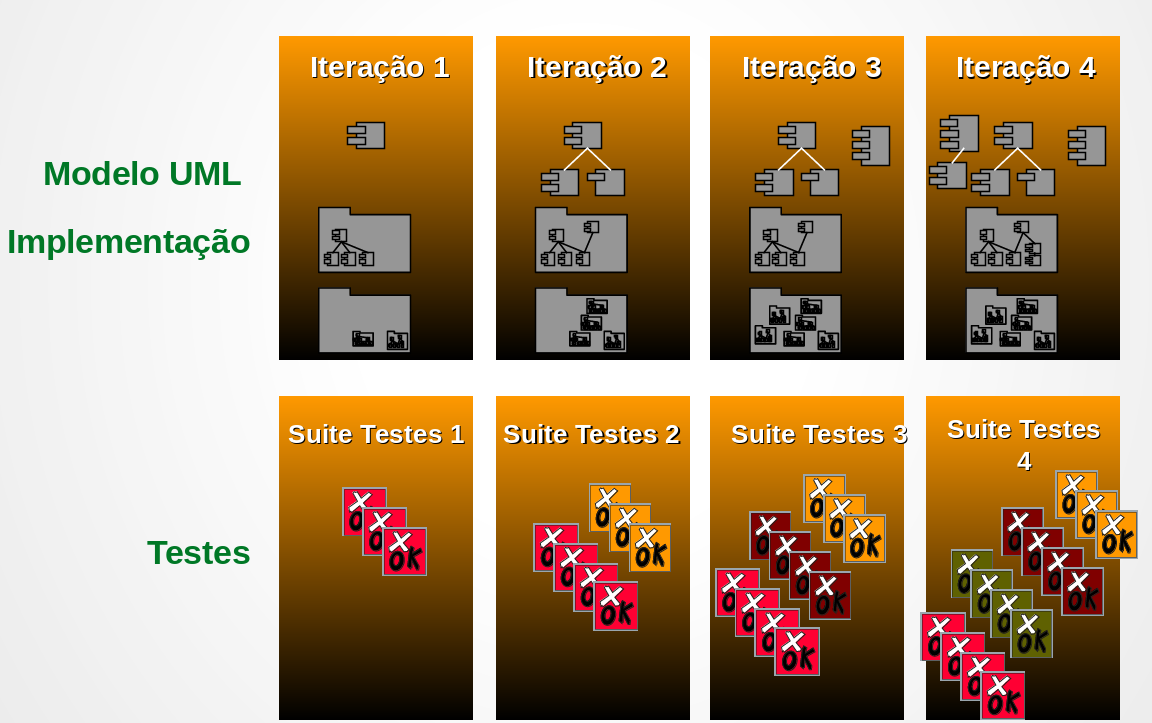
\includegraphics[width = 0.9\textwidth]{figs/fig16.png}
  \end{figure}
\end{frame}

\begin{frame}
\frametitle{O Teste no ciclo de vida do projeto}
\begin{figure}
   \centering
   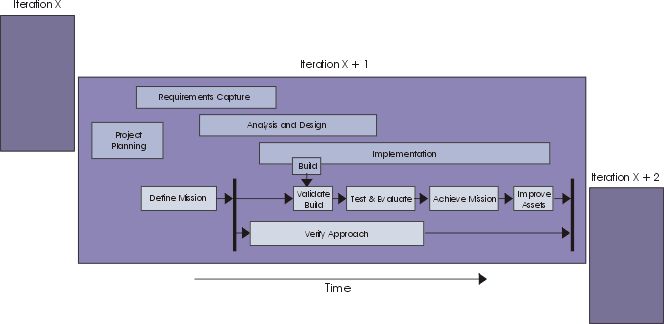
\includegraphics[width = 0.9\textwidth]{figs/fig17.png}
  \end{figure}
\end{frame}

\section{Gerencie Mudanças }
\begin{frame}
 \frametitle{Prática 3: Gerencie Mudanças }
 \begin{block}{Boas Práticas}
 \begin{itemize}
  \item Desenvolva Iterativamente
  \item Gerencie Requisitos
  \item Use arquitetura componentizada
  \item  Modele Visualmente (UML)	
  \item  Verifique Continuamente a Qualidade
  \item \textbf{Gerencie Mudanças}
 \end{itemize}
\end{block}
\end{frame}

\begin{frame}
\frametitle{O que você deve monitorar?}
 \begin{itemize}
  \item Área de trabalho para cada desenvolvedor
  \item Gerenciamento automatizado de integração e build
  \item Desenvolvimento paralelo
  \end{itemize}
\end{frame}


\begin{frame}
\frametitle{Aspectos do Gerenciamento da  Configuração}
 \begin{itemize}
  \item Gerenciamento de solicitação de mudança (CRM)
  \item Configuração do Status Reporting 
  \item Gerenciamento de Configuração (CM)
  \item Rastreamento das mudanças
  \item Seleção da versão
  \item Manufatura do software
  \end{itemize}
\end{frame}

\begin{frame}
 \frametitle{Gerenciamento de Requisitos}
 \begin{itemize}
  \item Tenha certeza que
  \begin{itemize}
   \item está resolvendo o problema correto
   \item está construindo os “builds” corretos
  \end{itemize}
  \item por meio de uma abordagem sistemática
  \begin{itemize}
   \item de levantamento dos problemas
   \item organizada
   \item documentada
   \item gerenciada 
   \end{itemize}

 \end{itemize}

\end{frame}

\begin{frame}
\frametitle{Cada prática reforça a necessidade da outra}
\begin{figure}
   \centering
   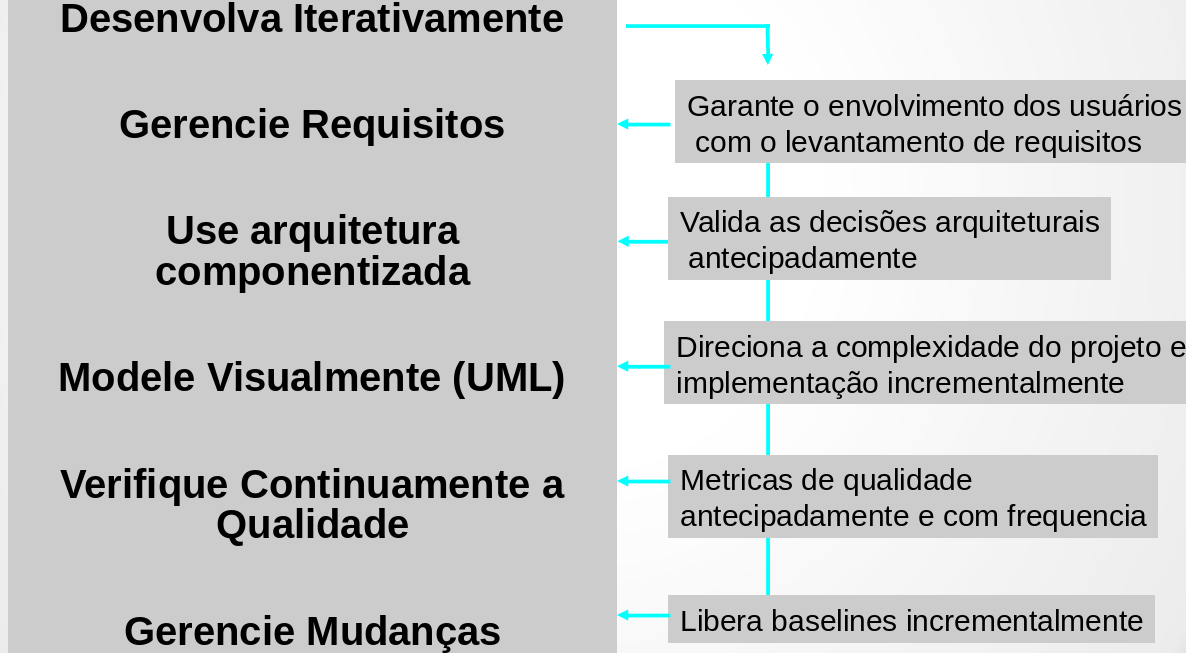
\includegraphics[width = 0.9\textwidth]{figs/fig18.png}
  \end{figure}
\end{frame}
\section{RUP no context das boas práticas}

\begin{frame}
 \frametitle{Propóstio de uma arquitetura robusta baseada em componentes}
  \begin{minipage}[t]{0.48\linewidth}
  \begin{itemize}
   \item Abordagem iterativa
  \item Guias para as atividades e artefatos
  \item Processo focado na arquitetura
  \item Os casos de uso direcionam o projeto e a implementação
  \item Modelos que abstraem o sistema
  \end{itemize}
 \end{minipage}
\begin{minipage}[t]{0.48\linewidth}
\textbf{RUP}
  \begin{figure}
   \centering
   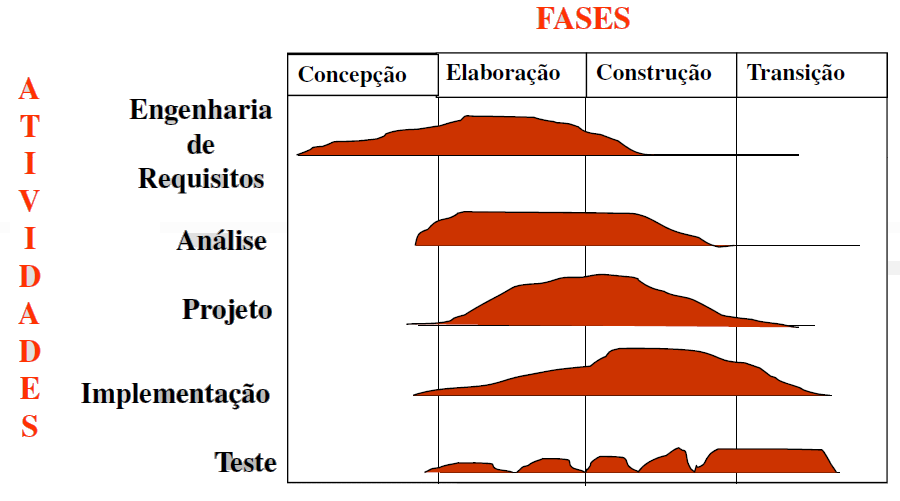
\includegraphics[width = 0.8\textwidth]{figs/fig19.png}
  \end{figure}
\end{minipage}

\end{frame}

\begin{frame}
 \frametitle{A definição de um processo}
\begin{block}{}
 Um processo define \textbf{Quem} está fazendo \textbf{O Que}, \textbf{Quando}, e \textbf{Como}, afim de alcançar um objetivo.
\end{block}

\end{frame}
\begin{frame}
 \frametitle{Estrutura do processo - Fases}
\begin{itemize}
 \item Rational Unified Process tem quatro fases:
 \begin{enumerate}
  \item \textbf{Iniciação} - Define o \textbf{escopo} do projeto
  \item \textbf{Elaboração} - Planeja o projeto,especifica as características, \textbf{define a baseline da arquitetura} 
  \item \textbf{Construção} - \textbf{constrói} o produto
  \item \textbf{Transição} - Transição do produto para \textbf{o usuário final}
 \end{enumerate}
\end{itemize}


\end{frame}

\begin{frame}
\frametitle{As fronteiras das fases definem os principais marcos}
\begin{figure}
   \centering
   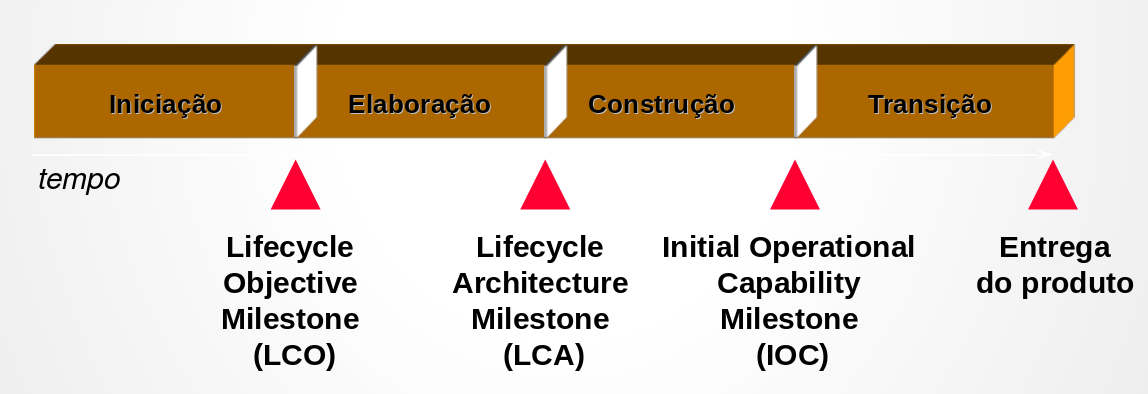
\includegraphics[width = 0.9\textwidth]{figs/fig20.png}
  \end{figure}
\end{frame}

\begin{frame}
\frametitle{Iterações e Fases}
\begin{figure}
   \centering
   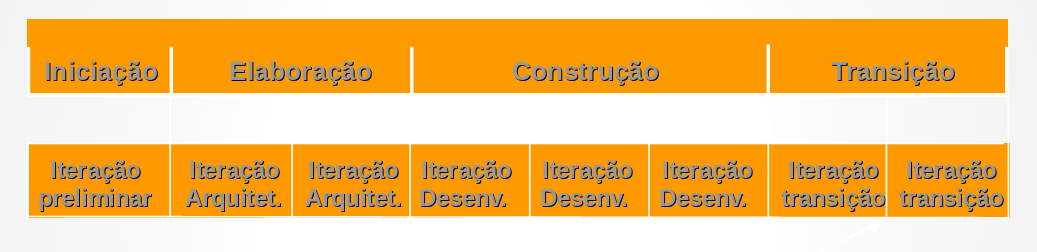
\includegraphics[width = 0.9\textwidth]{figs/fig21.png}
   \caption{Milestones secudários: Entregas}
  \end{figure}
  \begin{block}{}
   Uma iteração é uma sequencia distinta de atividades baseadas em um plano estabelecido e um critério de avaliação, que resulta em uma entrega executável (interna ou externa)
  \end{block}
\end{frame}

\begin{frame}
\frametitle{A abordagem iterativa}
\begin{figure}
   \centering
   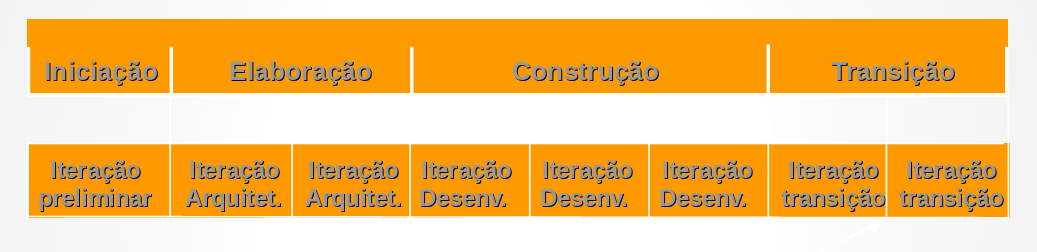
\includegraphics[width = 0.9\textwidth]{figs/fig21.png}
  \end{figure}
\end{frame}

\begin{frame}
\frametitle{As disciplinas produzem modelos}
\begin{figure}
   \centering
   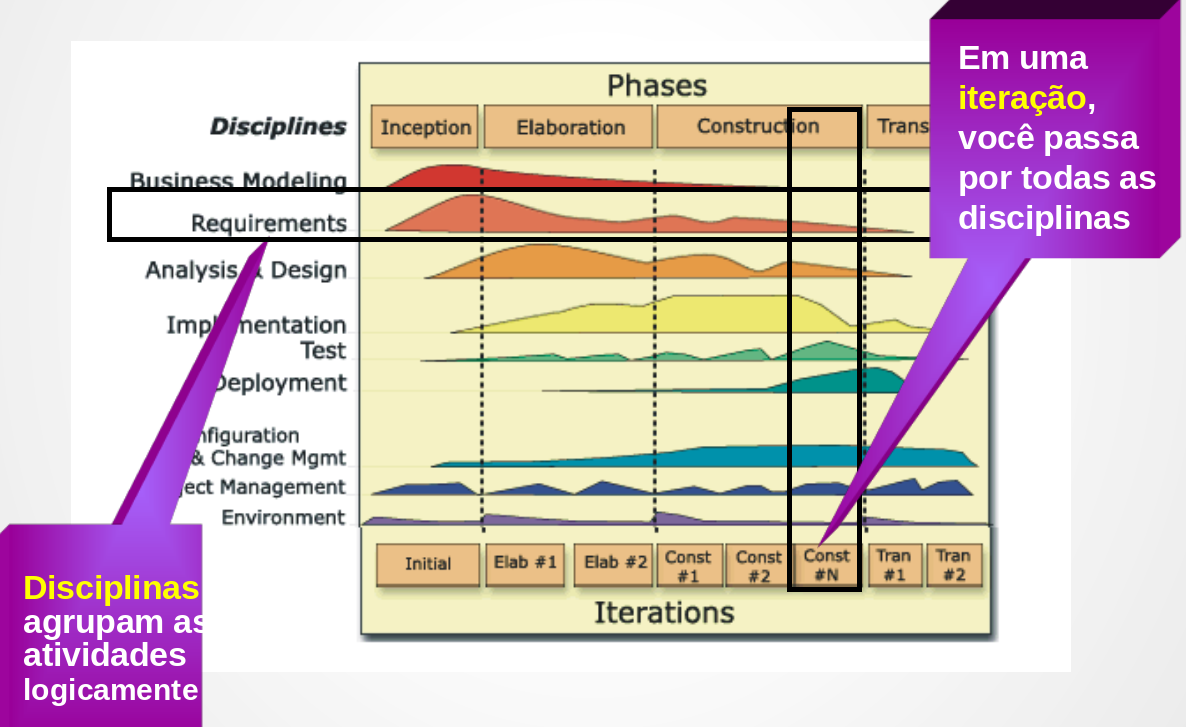
\includegraphics[width = 0.9\textwidth]{figs/fig22.png}
  \end{figure}
\end{frame}

\begin{frame}
\frametitle{As disciplinas guiam um desenvolvimento iterativo}
\begin{figure}
   \centering
   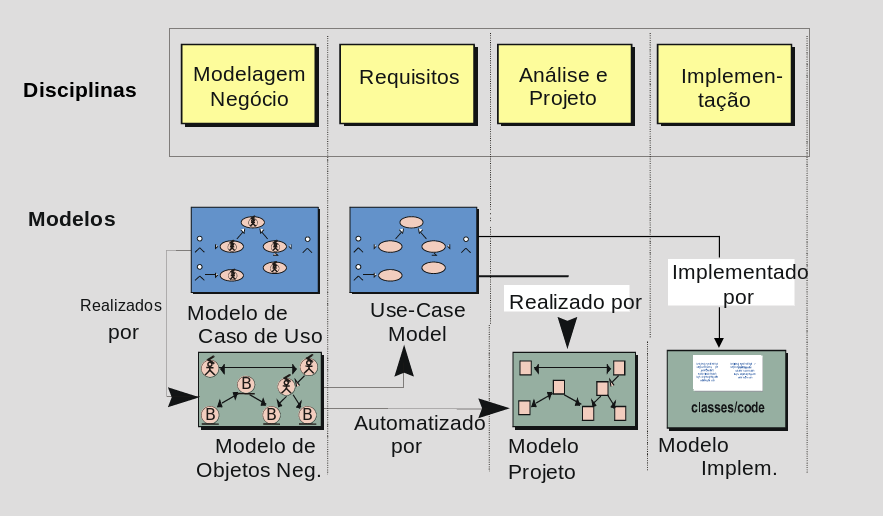
\includegraphics[width = 0.9\textwidth]{figs/fig23.png}
  \end{figure}
\end{frame}


\begin{frame}
\frametitle{Visão geral dos conceitos do RUP}
\begin{figure}
   \centering
   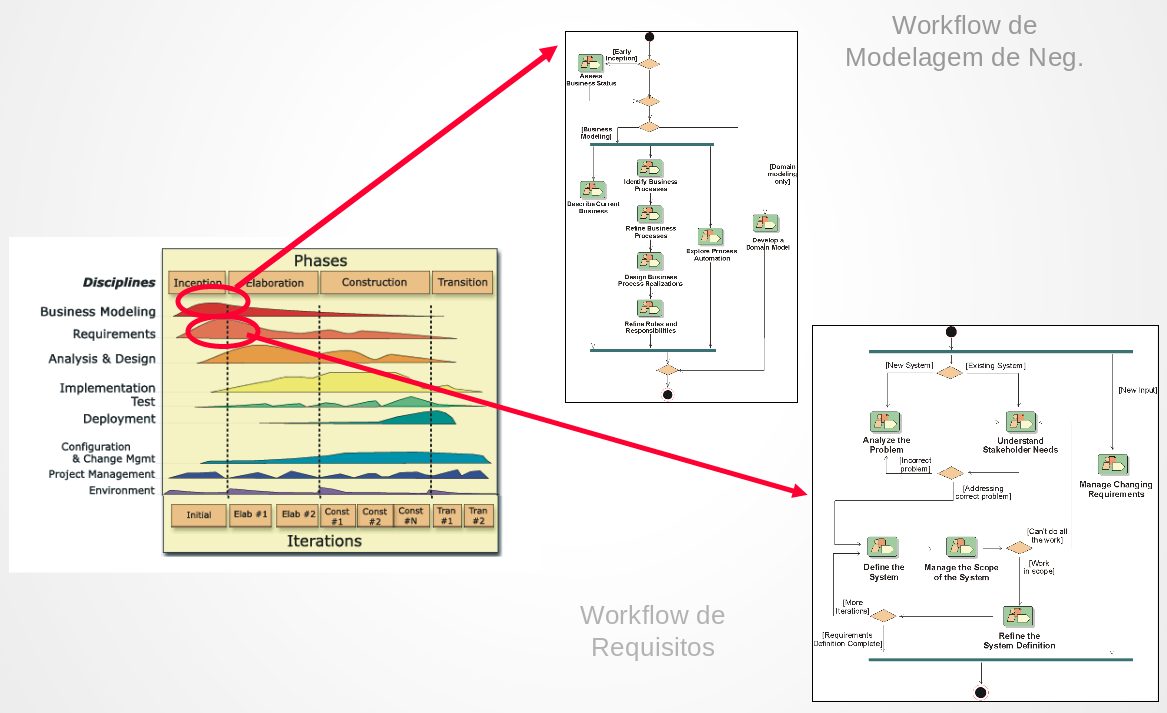
\includegraphics[width = 0.9\textwidth]{figs/fig24.png}
  \end{figure}
\end{frame}

\begin{frame}
 \frametitle{Revisão}
 \begin{itemize}
  \item As boas práticas guiam a engenharia de software tratando as causas raízes
  \item Cada práticas reforça a necessidade da outra
  \item Um processo guia uma equipe em: quem faz o que, quando e como
  \item O RUP é um mecanismo de alcançar as boas práticas
  \end{itemize}

\end{frame}

\begin{frame}
 \frametitle{Bibliografia da Aula}
 \begin{itemize}
  \item Udacity - Process Software Development
 \end{itemize}

\end{frame}
